%% BioMed_Central_Tex_Template_v1.06
%%                                      %
%  bmc_article.tex            ver: 1.06 %
%                                       %

%%IMPORTANT: do not delete the first line of this template
%%It must be present to enable the BMC Submission system to
%%recognise this template!!

%%%%%%%%%%%%%%%%%%%%%%%%%%%%%%%%%%%%%%%%%
%%                                     %%
%%  LaTeX template for BioMed Central  %%
%%     journal article submissions     %%
%%                                     %%
%%          <8 June 2012>              %%
%%                                     %%
%%                                     %%
%%%%%%%%%%%%%%%%%%%%%%%%%%%%%%%%%%%%%%%%%


%%%%%%%%%%%%%%%%%%%%%%%%%%%%%%%%%%%%%%%%%%%%%%%%%%%%%%%%%%%%%%%%%%%%%
%%                                                                 %%
%% For instructions on how to fill out this Tex template           %%
%% document please refer to Readme.html and the instructions for   %%
%% authors page on the biomed central website                      %%
%% http://www.biomedcentral.com/info/authors/                      %%
%%                                                                 %%
%% Please do not use \input{...} to include other tex files.       %%
%% Submit your LaTeX manuscript as one .tex document.              %%
%%                                                                 %%
%% All additional figures and files should be attached             %%
%% separately and not embedded in the \TeX\ document itself.       %%
%%                                                                 %%
%% BioMed Central currently use the MikTex distribution of         %%
%% TeX for Windows) of TeX and LaTeX.  This is available from      %%
%% http://www.miktex.org                                           %%
%%                                                                 %%
%%%%%%%%%%%%%%%%%%%%%%%%%%%%%%%%%%%%%%%%%%%%%%%%%%%%%%%%%%%%%%%%%%%%%

%%% additional documentclass options:
%  [doublespacing]
%  [linenumbers]   - put the line numbers on margins

%%% loading packages, author definitions

%\documentclass[twocolumn]{bmcart}% uncomment this for twocolumn layout and comment line below
\documentclass{bmcart}

%%% Load packages
%\usepackage{amsthm,amsmath}
%\RequirePackage{natbib}
%\RequirePackage{hyperref}
\usepackage[utf8]{inputenc} %unicode support
\usepackage{graphicx}
\usepackage{multirow}
%\usepackage[applemac]{inputenc} %applemac support if unicode package fails
%\usepackage[latin1]{inputenc} %UNIX support if unicode package fails


%%%%%%%%%%%%%%%%%%%%%%%%%%%%%%%%%%%%%%%%%%%%%%%%%
%%                                             %%
%%  If you wish to display your graphics for   %%
%%  your own use using includegraphic or       %%
%%  includegraphics, then comment out the      %%
%%  following two lines of code.               %%
%%  NB: These line *must* be included when     %%
%%  submitting to BMC.                         %%
%%  All figure files must be submitted as      %%
%%  separate graphics through the BMC          %%
%%  submission process, not included in the    %%
%%  submitted article.                         %%
%%                                             %%
%%%%%%%%%%%%%%%%%%%%%%%%%%%%%%%%%%%%%%%%%%%%%%%%%


%\def\includegraphic{}
%\def\includegraphics{}



%%% Put your definitions there:
\startlocaldefs
\endlocaldefs


%%% Begin ...
\begin{document}

%%% Start of article front matter
\begin{frontmatter}

\begin{fmbox}
\dochead{Research}

%%%%%%%%%%%%%%%%%%%%%%%%%%%%%%%%%%%%%%%%%%%%%%
%%                                          %%
%% Enter the title of your article here     %%
%%                                          %%
%%%%%%%%%%%%%%%%%%%%%%%%%%%%%%%%%%%%%%%%%%%%%%

\title{GNParser -- a Scientific Names Parser
  from Global Names Architecture Project}

%%%%%%%%%%%%%%%%%%%%%%%%%%%%%%%%%%%%%%%%%%%%%%
%%                                          %%
%% Enter the authors here                   %%
%%                                          %%
%% Specify information, if available,       %%
%% in the form:                             %%
%%   <key>={<id1>,<id2>}                    %%
%%   <key>=                                 %%
%% Comment or delete the keys which are     %%
%% not used. Repeat \author command as much %%
%% as required.                             %%
%%                                          %%
%%%%%%%%%%%%%%%%%%%%%%%%%%%%%%%%%%%%%%%%%%%%%%

\author[
   addressref={aff1},
   corref={aff1},                       % id of corresponding address, if any
   email={dmozzherin@gmail.com}
]{\inits{DYM}\fnm{Dmitry Y} \snm{Mozzherin}}
\author[                  % id's of addresses, e.g. {aff1,aff2}
   noteref={n1},% id's of article notes, if any
   email={alexander.myltsev@phystech.edu}   % email address
]{\inits{AAM}\fnm{Alexander A} \snm{Myltsev}}
\author[
   email={dpatterson.mbl@gmail.com}
]{\inits{DJP}\fnm{David J} \snm{Patterson}}

%%%%%%%%%%%%%%%%%%%%%%%%%%%%%%%%%%%%%%%%%%%%%%
%%                                          %%
%% Enter the authors' addresses here        %%
%%                                          %%
%% Repeat \address commands as much as      %%
%% required.                                %%
%%                                          %%
%%%%%%%%%%%%%%%%%%%%%%%%%%%%%%%%%%%%%%%%%%%%%%

\address[id=aff1]{%                          % unique id
  \orgname{Marine Biological Laboratory},    % university, etc
  \street{7 MBL Street},                     %
  \postcode{02543}                           % post or zip code
  \city{Woods Hole},                         % city
  \cny{US}                                   % country
}

%%%%%%%%%%%%%%%%%%%%%%%%%%%%%%%%%%%%%%%%%%%%%%
%%                                          %%
%% Enter short notes here                   %%
%%                                          %%
%% Short notes will be after addresses      %%
%% on first page.                           %%
%%                                          %%
%%%%%%%%%%%%%%%%%%%%%%%%%%%%%%%%%%%%%%%%%%%%%%

\begin{artnotes}
%\note{Sample of title note}     % note to the article
\note[id=n1]{Equal contributor} % note, connected to author
\end{artnotes}

\end{fmbox}% comment this for two column layout

%%%%%%%%%%%%%%%%%%%%%%%%%%%%%%%%%%%%%%%%%%%%%%
%%                                          %%
%% The Abstract begins here                 %%
%%                                          %%
%% Please refer to the Instructions for     %%
%% authors on http://www.biomedcentral.com  %%
%% and include the section headings         %%
%% accordingly for your article type.       %%
%%                                          %%
%%%%%%%%%%%%%%%%%%%%%%%%%%%%%%%%%%%%%%%%%%%%%%

\begin{abstractbox}

\begin{abstract} % abstract
Modern biology is unthinkable without names based on Linnaean nomenclature.
Names of organisms are pervasive, they are metadata which allows to communicate
information in biodiversity, ecology, molecular biology and medicine and many
other fields. However indexing and organizing such information via scientific
names is challenging for several reasons. One of the most significant ones:
names exist in a variety of alternative forms like for example “Aedes
(Cancraedes) thurmanae” and “Aedes thurmanae Mattingly, 1958”, therefore a
simple string matching is insufficient for finding names in a majority of
cases. Global Names Parser breaks names into semantic elements, allowing to
normalize them into “canonical forms” (Aedes thurmanae for both examples). It
reveals elements ‘hidden’ within names (like ranks, years of publication, names
of authors etc). Global Names Parser is written in Scala, a Java Virtual
Machine language. It is fast (millions of names/hour per CPU), can be used in
any JVM-based language (Scala, Java, JRuby, Rengin, Jythion etc.), and accurate
(X/X Precision/Recall ratio). The program is based on Parsing Expression
Grammar which provides additional flexibility and is able to deal with the most
complex name strings.
\end{abstract}

%%%%%%%%%%%%%%%%%%%%%%%%%%%%%%%%%%%%%%%%%%%%%%
%%                                          %%
%% The keywords begin here                  %%
%%                                          %%
%% Put each keyword in separate \kwd{}.     %%
%%                                          %%
%%%%%%%%%%%%%%%%%%%%%%%%%%%%%%%%%%%%%%%%%%%%%%

\begin{keyword}
\kwd{biodiversity}
\kwd{scientific name}
\kwd{parser}
\end{keyword}

% MSC classifications codes, if any
%\begin{keyword}[class=AMS]
%\kwd[Primary ]{}
%\kwd{}
%\kwd[; secondary ]{}
%\end{keyword}

\end{abstractbox}
%
%\end{fmbox}% uncomment this for twcolumn layout

\end{frontmatter}

%%%%%%%%%%%%%%%%%%%%%%%%%%%%%%%%%%%%%%%%%%%%%%
%%                                          %%
%% The Main Body begins here                %%
%%                                          %%
%% Please refer to the instructions for     %%
%% authors on:                              %%
%% http://www.biomedcentral.com/info/authors%%
%% and include the section headings         %%
%% accordingly for your article type.       %%
%%                                          %%
%% See the Results and Discussion section   %%
%% for details on how to create sub-sections%%
%%                                          %%
%% use \cite{...} to cite references        %%
%%  \cite{koon} and                         %%
%%  \cite{oreg,khar,zvai,xjon,schn,pond}    %%
%%  \nocite{smith,marg,hunn,advi,koha,mouse}%%
%%                                          %%
%%%%%%%%%%%%%%%%%%%%%%%%%%%%%%%%%%%%%%%%%%%%%%

%%%%%%%%%%%%%%%%%%%%%%%%% start of article main body
% <put your article body there>

\section*{Introduction}

Throughout the paper we distinguish between two terms -- name and name-string.
Name is an entity which can be mapped to a nomenclatural event. Nomenclatural
event is a declaration of a name in a code-compliant publication. A name can be
expressed through many spelling variants, some are well-formed and code
compliant, and others are not. These spelling variants we call name-strings.
Every scientific name can be expressed through a large amount of name-strings
(Table 1).  There are millions of scientific names and billions of possible
"correct" name strings. When we talk about 'code-compliancy' we mean compliance
with codes of nomenclature (ICZN, ICBN, Bacteria, Viruses, cultivated plants,
Biocode, Phylocode). Codes of nomenclature determine rules for composing
scientific names from infraspecific to family level. Other levels comply with
community practices.

The names of organisms are invaluable in the world of big biodiversity data
because they can be used as near universal metadata to index, organize and
interconnect distributed information (Patterson et al., 2010). Nevertheless,
use of names for informatics purposes presents an array of problems. Many of
these problems can be solved by parsing, or deducing the semantic meaning of
words occurred in the name-strings.

How can we match all the possible name-strings of the same name? Parsing allows
to remove the most variable parts (like authorship, rank, a year of
publication) and compare names by the most stable component -- the canonical
form of a name. Such approach brings us to another problem -- the same
canonical form may be used for more than one taxon or concept in case of
homonyms, or subtleties of intraspecific ranks. Analysis of ranks and the
authors revealed in the name-strings by parser helps to separate homonyms and
similar names from each  other.

\begin{table}[h!]
  \begin{center}
    \begin{tabular}{| l | c |}
    \hline
    Carex scirpoidea convoluta &
    \multirow{25}{*}{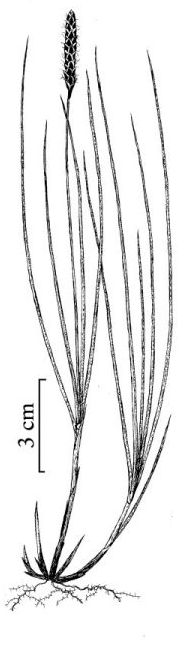
\includegraphics[scale=0.3]{images/carex.png}} \\
    Carex scirpoidea var. convoluta & \\
    Carex scirpoidea subsp. convoluta & \\
    Carex scirpoidea convoluta Gardner & \\
    Carex scirpoidea convoluta Kükenth. & \\
    Carex scirpoidea var. convoluta Kuk. & \\
    Carex scirpoidea var. convoluta Kük. & \\
    Carex scirpoidea var. convoluta Kükenth. & \\
    Carex scirpoidea var. convoluta Kükenthal & \\
    Carex scirpoidea Michx. var. convoluta Kük. & \\
    Carex scirpoidea ssp. convoluta (Kük.) Dunlop & \\
    Carex scirpoidea Michx. var. convoluta Kükenth. & \\
    Carex scirpoidea subsp. convoluta (Kük.) Dunlop & \\
    Carex scirpoidea ssp. convoluta (Kukenth.) Dunlop & \\
    Carex scirpoidea Michaux var. convoluta Kükenthal & \\
    Carex scirpoidea subsp. convoluta (Kük.) D.A.Dunlop & \\
    Carex scirpoidea subsp. convoluta (Kük.) D.A. Dunlop & \\
    Carex scirpoidea Michx. ssp. convoluta (Kük.) Dunlop & \\
    Carex scirpoidea subsp. convoluta (Kuk.) D. A. Dunlop & \\
    Carex scirpoidea Michx. subsp. convoluta (Kük.) Dunlop & \\
    Carex scirpoidea Michx. ssp. convoluta (Kükenth.) Dunlop & \\
    Carex scirpoidea subsp. convoluta (Kükenthal) D.A. Dunlop & \\
    Carex scirpoidea Michx. subsp. convoluta (Kük.) D.A.Dunlop & \\
    Carex scirpoidea Michx. subsp. convoluta (Kük.) D.A. Dunlop & \\
    Carex scirpoidea subsp. convoluta (Kükenthal 1909) D.A. Dunlop 1998 & \\
    \hline
    \end{tabular}
  \end{center}

  \caption{Some legitimate versions of the scientific name for the Northern
    Bulrush or Singlespike sedge.  The genus (Carex), species (scirpoidea), and
    subspecies (convoluta) may be annotated (var. subsp., and ssp.) or have the
    name of the original authority for the subspecies (Kükenthal), the species
    (Michaux), the combination (Dunlop), sometimes abbreviated and with or
    without dates. Image courtesy of \cite{FNA2002}.}

\end{table}

A significant number of biodiversity informatics projects (EOL, GBIF, CoL,
WoRMS, iDigBio, VetNet) aggregate information from many different sources.
Resulting name-strings are inconsistent in their format. Parsed names can be
normalized to the same style. Some name strings are not properly formed, other
contain annotations which are not part of the name. There are also “surrogate
names” -- they depict organisms which were not fully identified and mapped to a
formally described taxon, instead they were associated with a name string that
narrows down identification choices to some higher clade. Parser helps to
recognize such names and mark them as surrogate name-strings.

After parsing of a large name-string collection a researcher can collect all
the semantic data, and use it as a basis for statistical analysis, or for
practical purposes, for example for introducing search by authors name, year of
publication, species epithet etc. If a name-string cannot be ingested by a high
quality parser, the string is almost certainly not a well-formed scientific
name.

Due to intrinsic diversity of name-strings a simple string matching by
automated systems is not powerful enough to link distributed big data to
scientific names. This problem can be addressed by promoting a rigid standard
restricting each name to a single name-string, or through reconciliation. The
former strategy would require a costly international coordination, would not
eliminate future human mistakes, it cannot be applied to older documents, does
not allow for multiple points of view, nor for changes in taxonomic
perspective.  The reconciliation process involves folding of all known
name-strings into lexical groups.  This requires that we collate all synonyms
and other identifiers, as well as all variant spellings and representations of
names. Parsing is a necessary component of name reconciliation.

A second challenge is to replace old names with ones that are endorsed by
taxonomic authorities - this is a process referred to as resolution. Resolution
requires an up to date high quality taxonomic and nomenclatural data to map a
reconciled name-string to the currently used name/names. This process normally
does not include a parsing step.

Through the early history of biodiversity problem of parsing had been usually
addressed by a home-grown scripts running regular expressions (uBio something
else as an example) or by manual splitting of a name into its canonical form
and the authorship part. Both approaches proved to be limited. Regular
expressions are cumbersome and impractical when dealing with complex
name-strings, especially hybrids. Manual approach is error-prone, expensive,
slow and inflexible.

In 2008 we decided to create a specialized parsing library "biodiversity"
written in Ruby and based on Parsing Expression Grammar (PEG) methodology. We
used an excellent TreeTop Ruby library as an underlying PEG implementation. PEG
is well suited for recursive texts with formally defined grammars. Scientific
names follow rules of nomenclatural codes, and therefore order and
capitalization of elements in the name are well structured. Names can be quite
complex and recursive, for example hybrid name strings contain more than one
name, or infraspecies names might have authorship attached to both specific and
infraspecific parts of the name. Authorship itself is quite complex and can
include original authors who described a name, authors of a new combination, or
authors who made a name, but did not publish it.

We found that PEG approach allows us to solve all these complexity gracefully.
From other side PEG gave us enough flexibility to incorporate edge cases and
common mistakes in formation of names. The library biodiversity enjoyed a
noticeable popularity. At the time of writing it had been downloaded x number
of times, it is used by many reconciliation sites: Canadian Register of MArine
Species (CARMS) \cite{carms}, the iPlant TNRS \cite{iplant}, World Registry of
Marine Species (WoRMS) \cite{worms}.  Biodiversity parser was marked as the
most popular bio-library in Ruby language.

In 2009 GBIF created another parser library written in Java (name-parser). It
is loosely based on the test suite of "biodiversity" Ruby parser, and is the
most popular regular expression-based approach to the parsing problem.

We considered biodiversity parser library to be a working prototype -- a
playground which allowed us to identify parsing problems and implement
solutions for them. We also found that PEG is very well suited for breaking
scientific names into semantic elements. In 2015 we decided to use everything
we learned and create a new version of parser in Scala with underlying PEG
library -- parboiled2.

Scala is a strongly typed language built from the ground up as a combination of
object oriented and functional programming paradigms. One of the main features
of functional programming is preservation of immutable state, as a result it is
possible to run several parts of program in parallell without danger of
modifying state. Scala creates a rare flexibility of approaches to solve
computational problems. Scala had been written on Java Virtual Machine. It
means that the vast resources developed in Java are easily accessible in Scala.
And vice versa -- the libraries we produce can be used in a plethora of
languages (Java, Jython, Renjin, JRuby etc.). Scala, is a language designed for
scalability. Projects like Akka and Spark create flexibility of approaches in
concurrency and parallelization, allowing to execute code on many CPU and
computers at the same time, dramatically reducing response time for large
computational tasks.

The library parboiled2 had been initiated by one of the authors of this
manuscript, Alexander Myltsev in 2013 while participating in the Google Summer
of Code project initiated by TypeSafe organization. Alexander also had been the
major contributor in gnparser code.

%%%%%%%%%%%%%%%%%%%%%%%%%%%%%%%%%%%%%%%%%%%%%%%%%%%%%%%%%%%%%
%%                  The Bibliography                       %%
%%                                                         %%
%%  Bmc_mathpys.bst  will be used to                       %%
%%  create a .BBL file for submission.                     %%
%%  After submission of the .TEX file,                     %%
%%  you will be prompted to submit your .BBL file.         %%
%%                                                         %%
%%                                                         %%
%%  Note that the displayed Bibliography will not          %%
%%  necessarily be rendered by Latex exactly as specified  %%
%%  in the online Instructions for Authors.                %%
%%                                                         %%
%%%%%%%%%%%%%%%%%%%%%%%%%%%%%%%%%%%%%%%%%%%%%%%%%%%%%%%%%%%%%

% if your bibliography is in bibtex format, use those commands:
\bibliographystyle{bmc-mathphys} % Style BST file
\bibliography{gnparser.bib}      % Bibliography file (usually '*.bib' )

% or include bibliography directly:
% \begin{thebibliography}
% \bibitem{b1}
% \end{thebibliography}

\end{document}
